\subsection{Standard Perturbation Theory Validation (ex 2)}

To validate the second-order Standard Perturbation Theory (SPT) module, numerical tests were conducted on an $N_g^3 = 128^3$ grid with physical box length $L = 500\,h^{-1}\mathrm{Mpc}$ under two distinct linear variance regimes:
    \begin{enumerate}
        \item \textbf{Strong Coupling Regime ($\sigma_1^2 \approx 0.4613$):} 
        Designed for visualizing the spatial non-linear clustering in 2D density slices and the 1D power spectrum enhancement $P_{\mathrm{tot}}(k) = P_1(k) + P_{22}(k) + 2 P_{13}(k)$, yielding a total non-linear variance of $\sigma_{\mathrm{tot}}^2 \approx 0.9233$.
        
        \item \textbf{Weakly Non-Linear Regime ($\sigma_1^2 \approx 4.6116 \times 10^{-3}$):} 
        Adopted for rigorous perturbative comparison of the bispectrum and reduced skewness against tree-level analytical predictions, avoiding higher-order breakdown.
    \end{enumerate}

\subsubsection{Density Slices and 1D Power Spectrum Enhancement}

Figure~\ref{fig:spt_slices} shows the spatial density contrast, and Figure~\ref{fig:spt_pk_1d} shows the 1D power spectrum generated in the strong coupling regime.
    \begin{figure}[htbp]
            \centering
            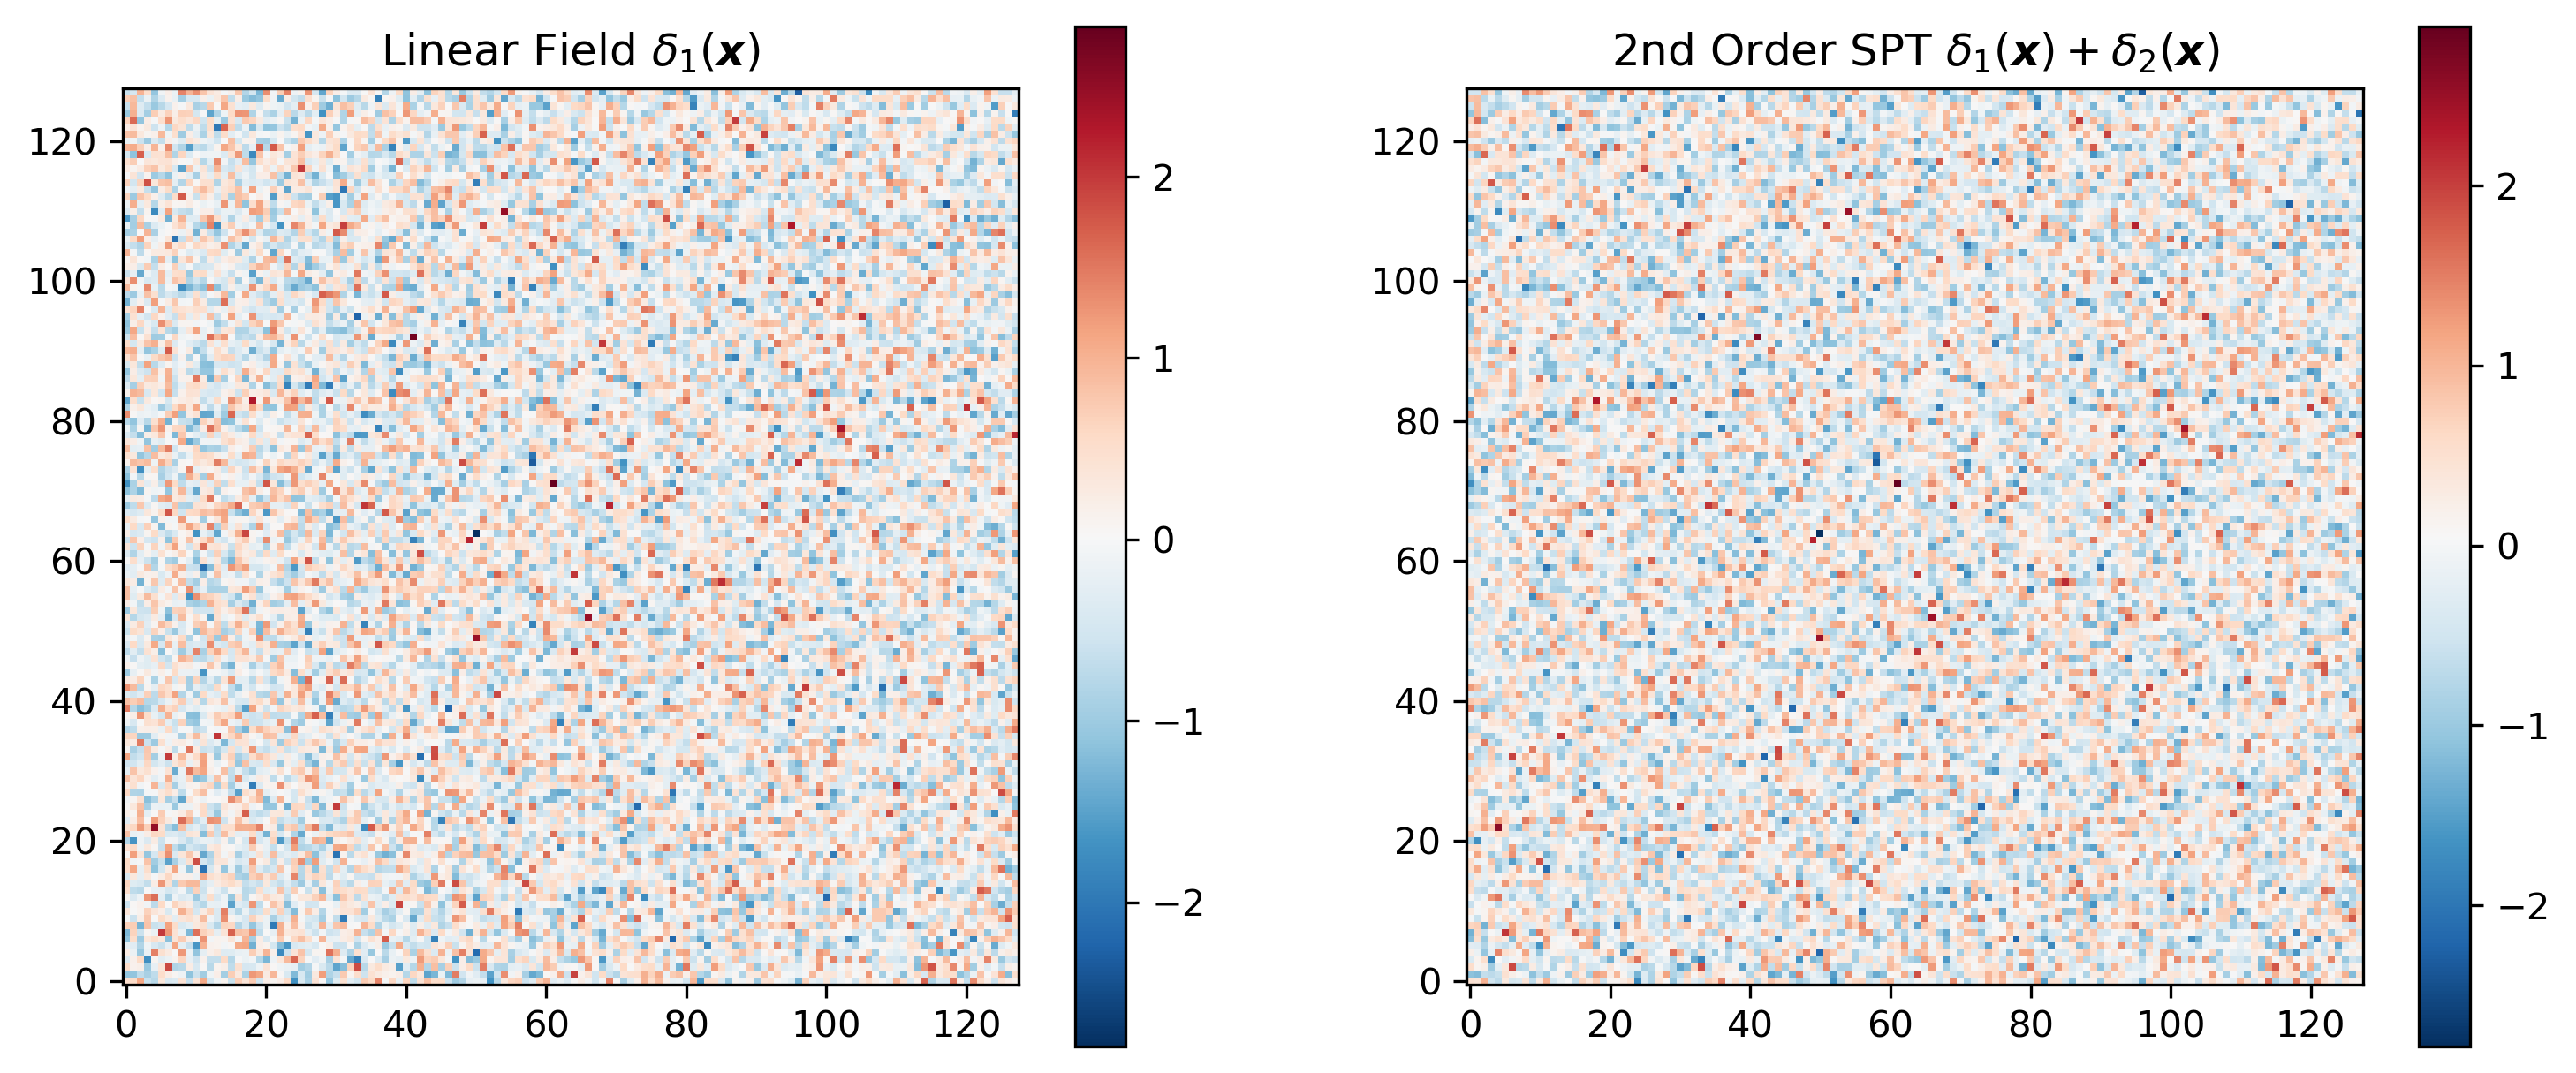
\includegraphics[width=0.9\textwidth]{New_Figures/Test_20261106_190746_Linear_Vs_2ndO_SPT.png}
            \caption{Linear density $\delta_1(\mathbf{x})$ vs. 2nd-order SPT $\delta_1(\mathbf{x}) + \delta_2(\mathbf{x})$.}
            \label{fig:spt_slices}
    \end{figure}

    \begin{figure}[htbp]
            \centering
            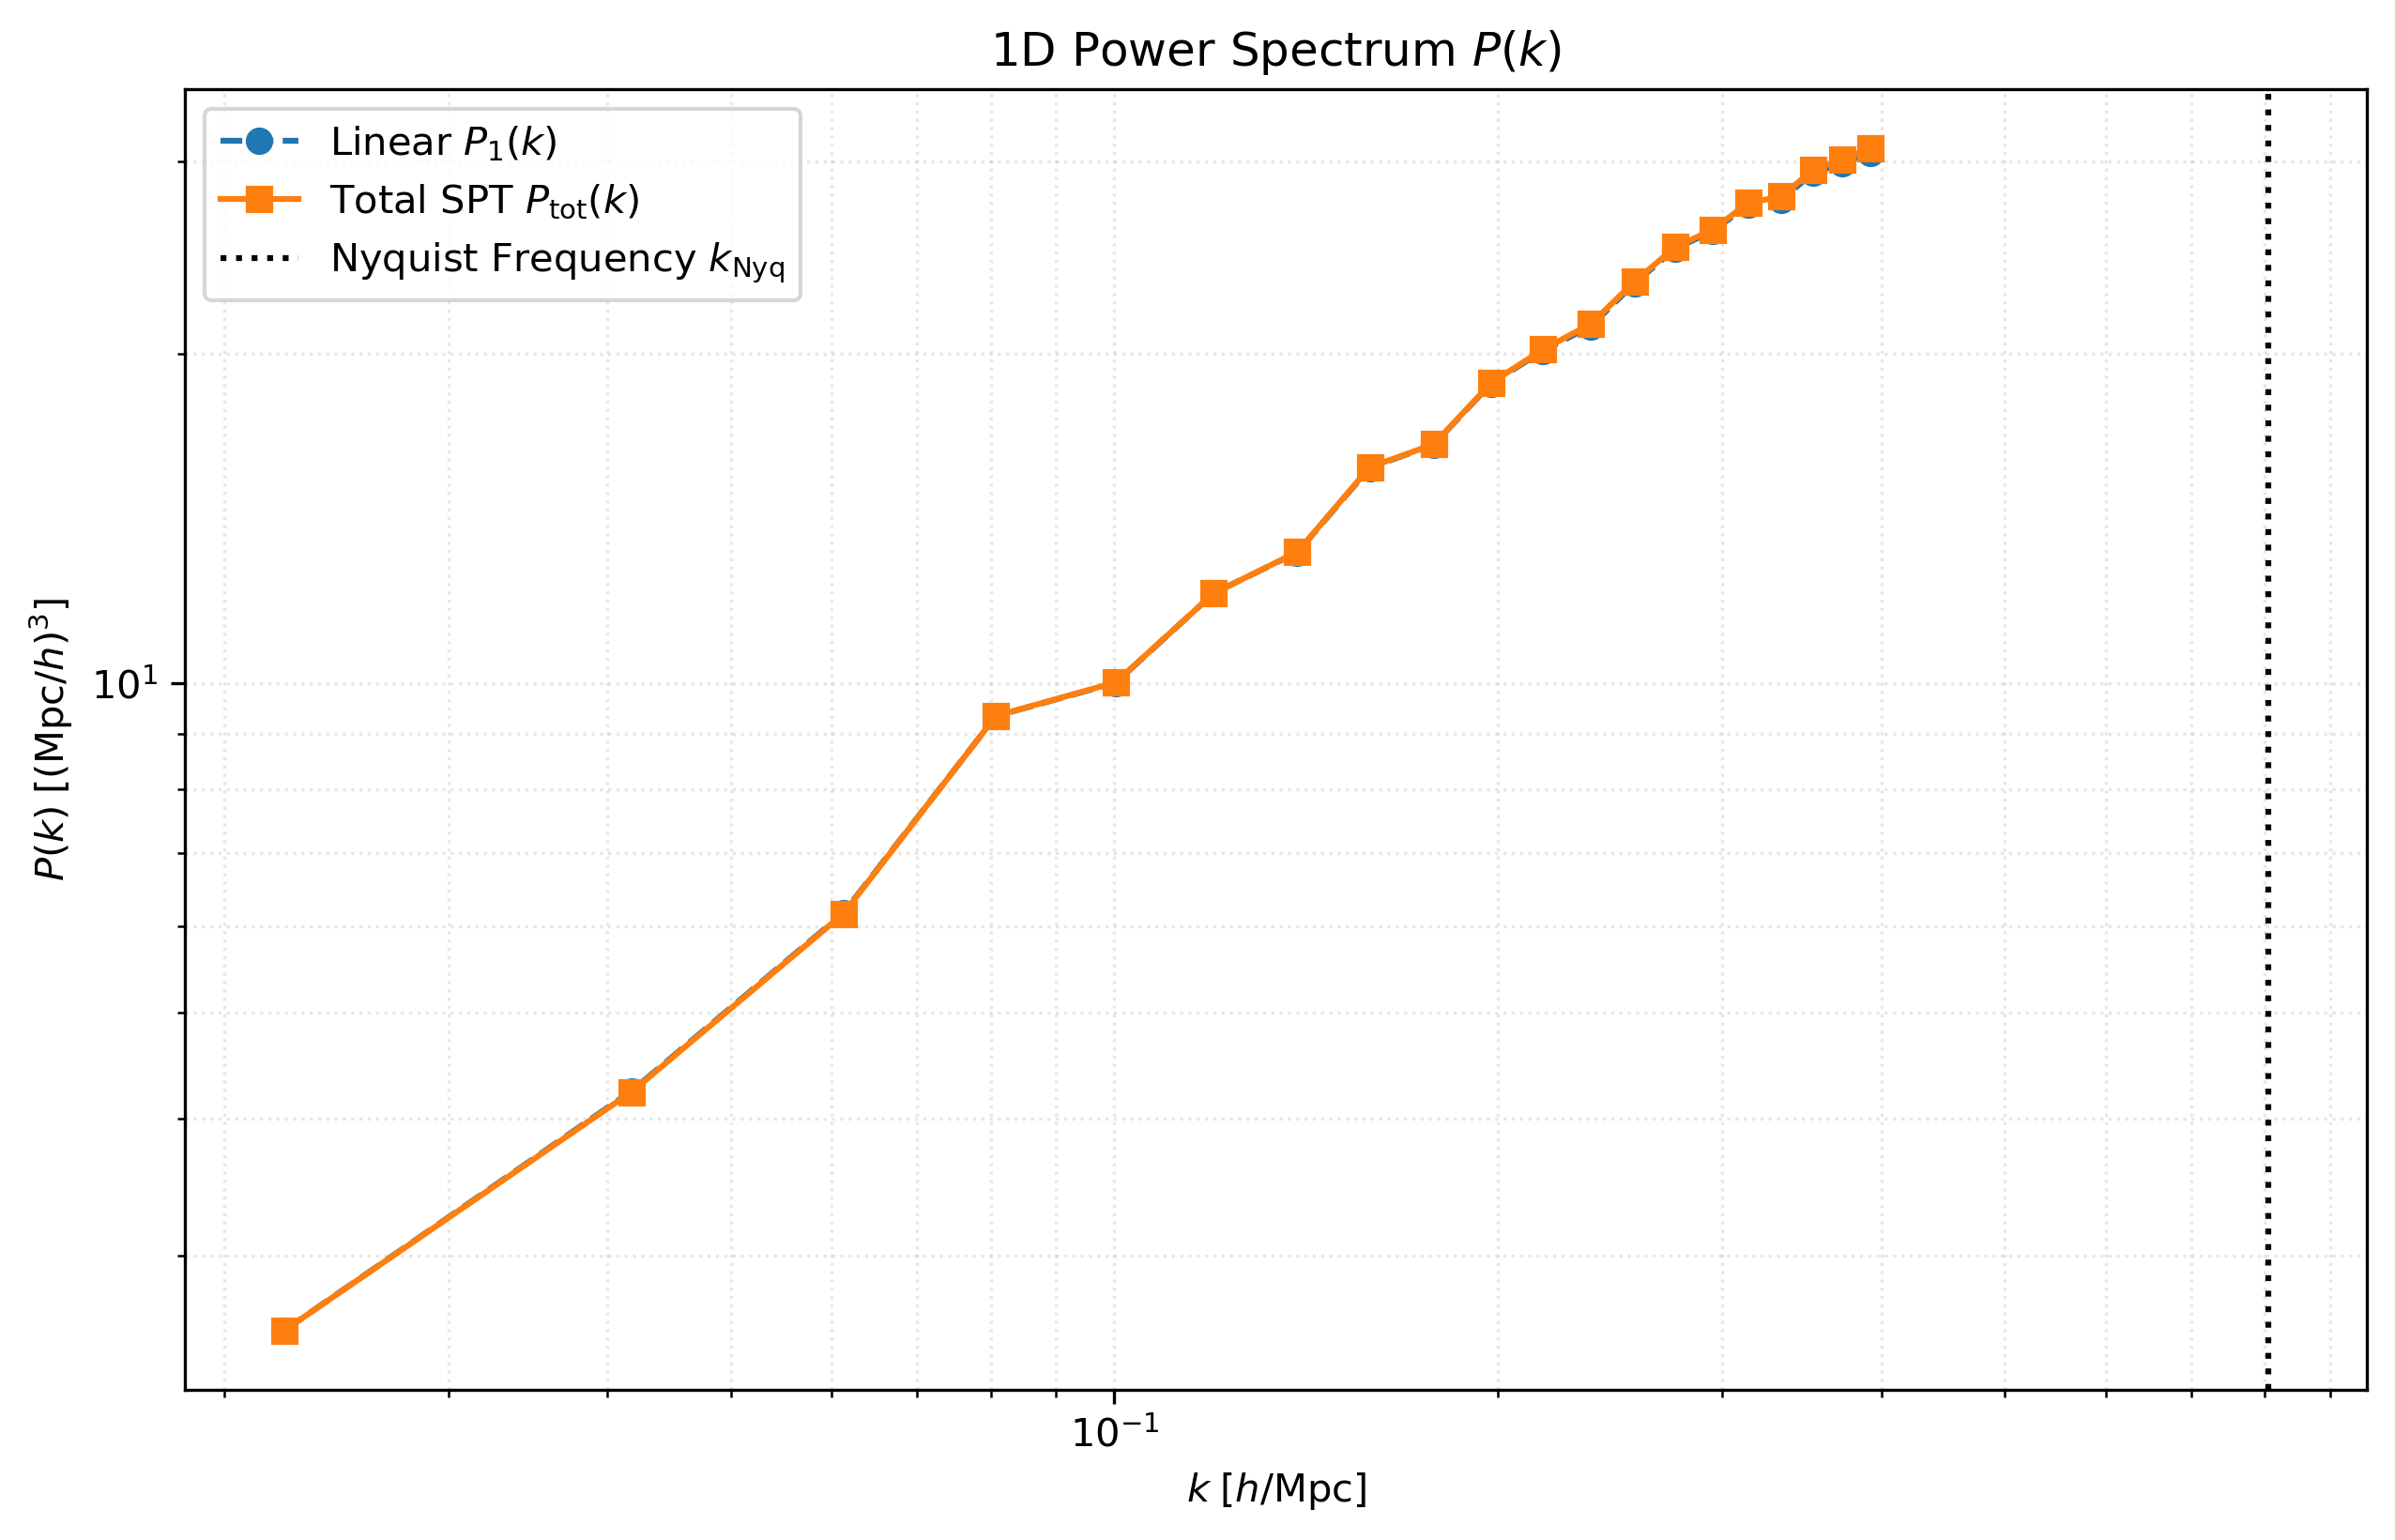
\includegraphics[width=0.8\textwidth]{New_Figures/Test_20261106_190746_Pk_1D_comparison.png}
            \caption{1D matter power spectrum $P_1(k)$ vs. $P_{\mathrm{tot}}(k)$.}
            \label{fig:spt_pk_1d}
    \end{figure}
    
Advection and tidal shear interactions in $\delta_2(\mathbf{x})$ assemble mass into localized, high-density structures (Figure~\ref{fig:spt_slices}), resulting in systematic power enhancement in $P_{\mathrm{tot}}(k)$ relative to linear theory across all resolved scales up to $k_{\mathrm{Nyq}}$ (Figure~\ref{fig:spt_pk_1d}).

\subsubsection{Higher-Order Non-Gaussian Statistics}

    \begin{figure}[H]
        \centering
        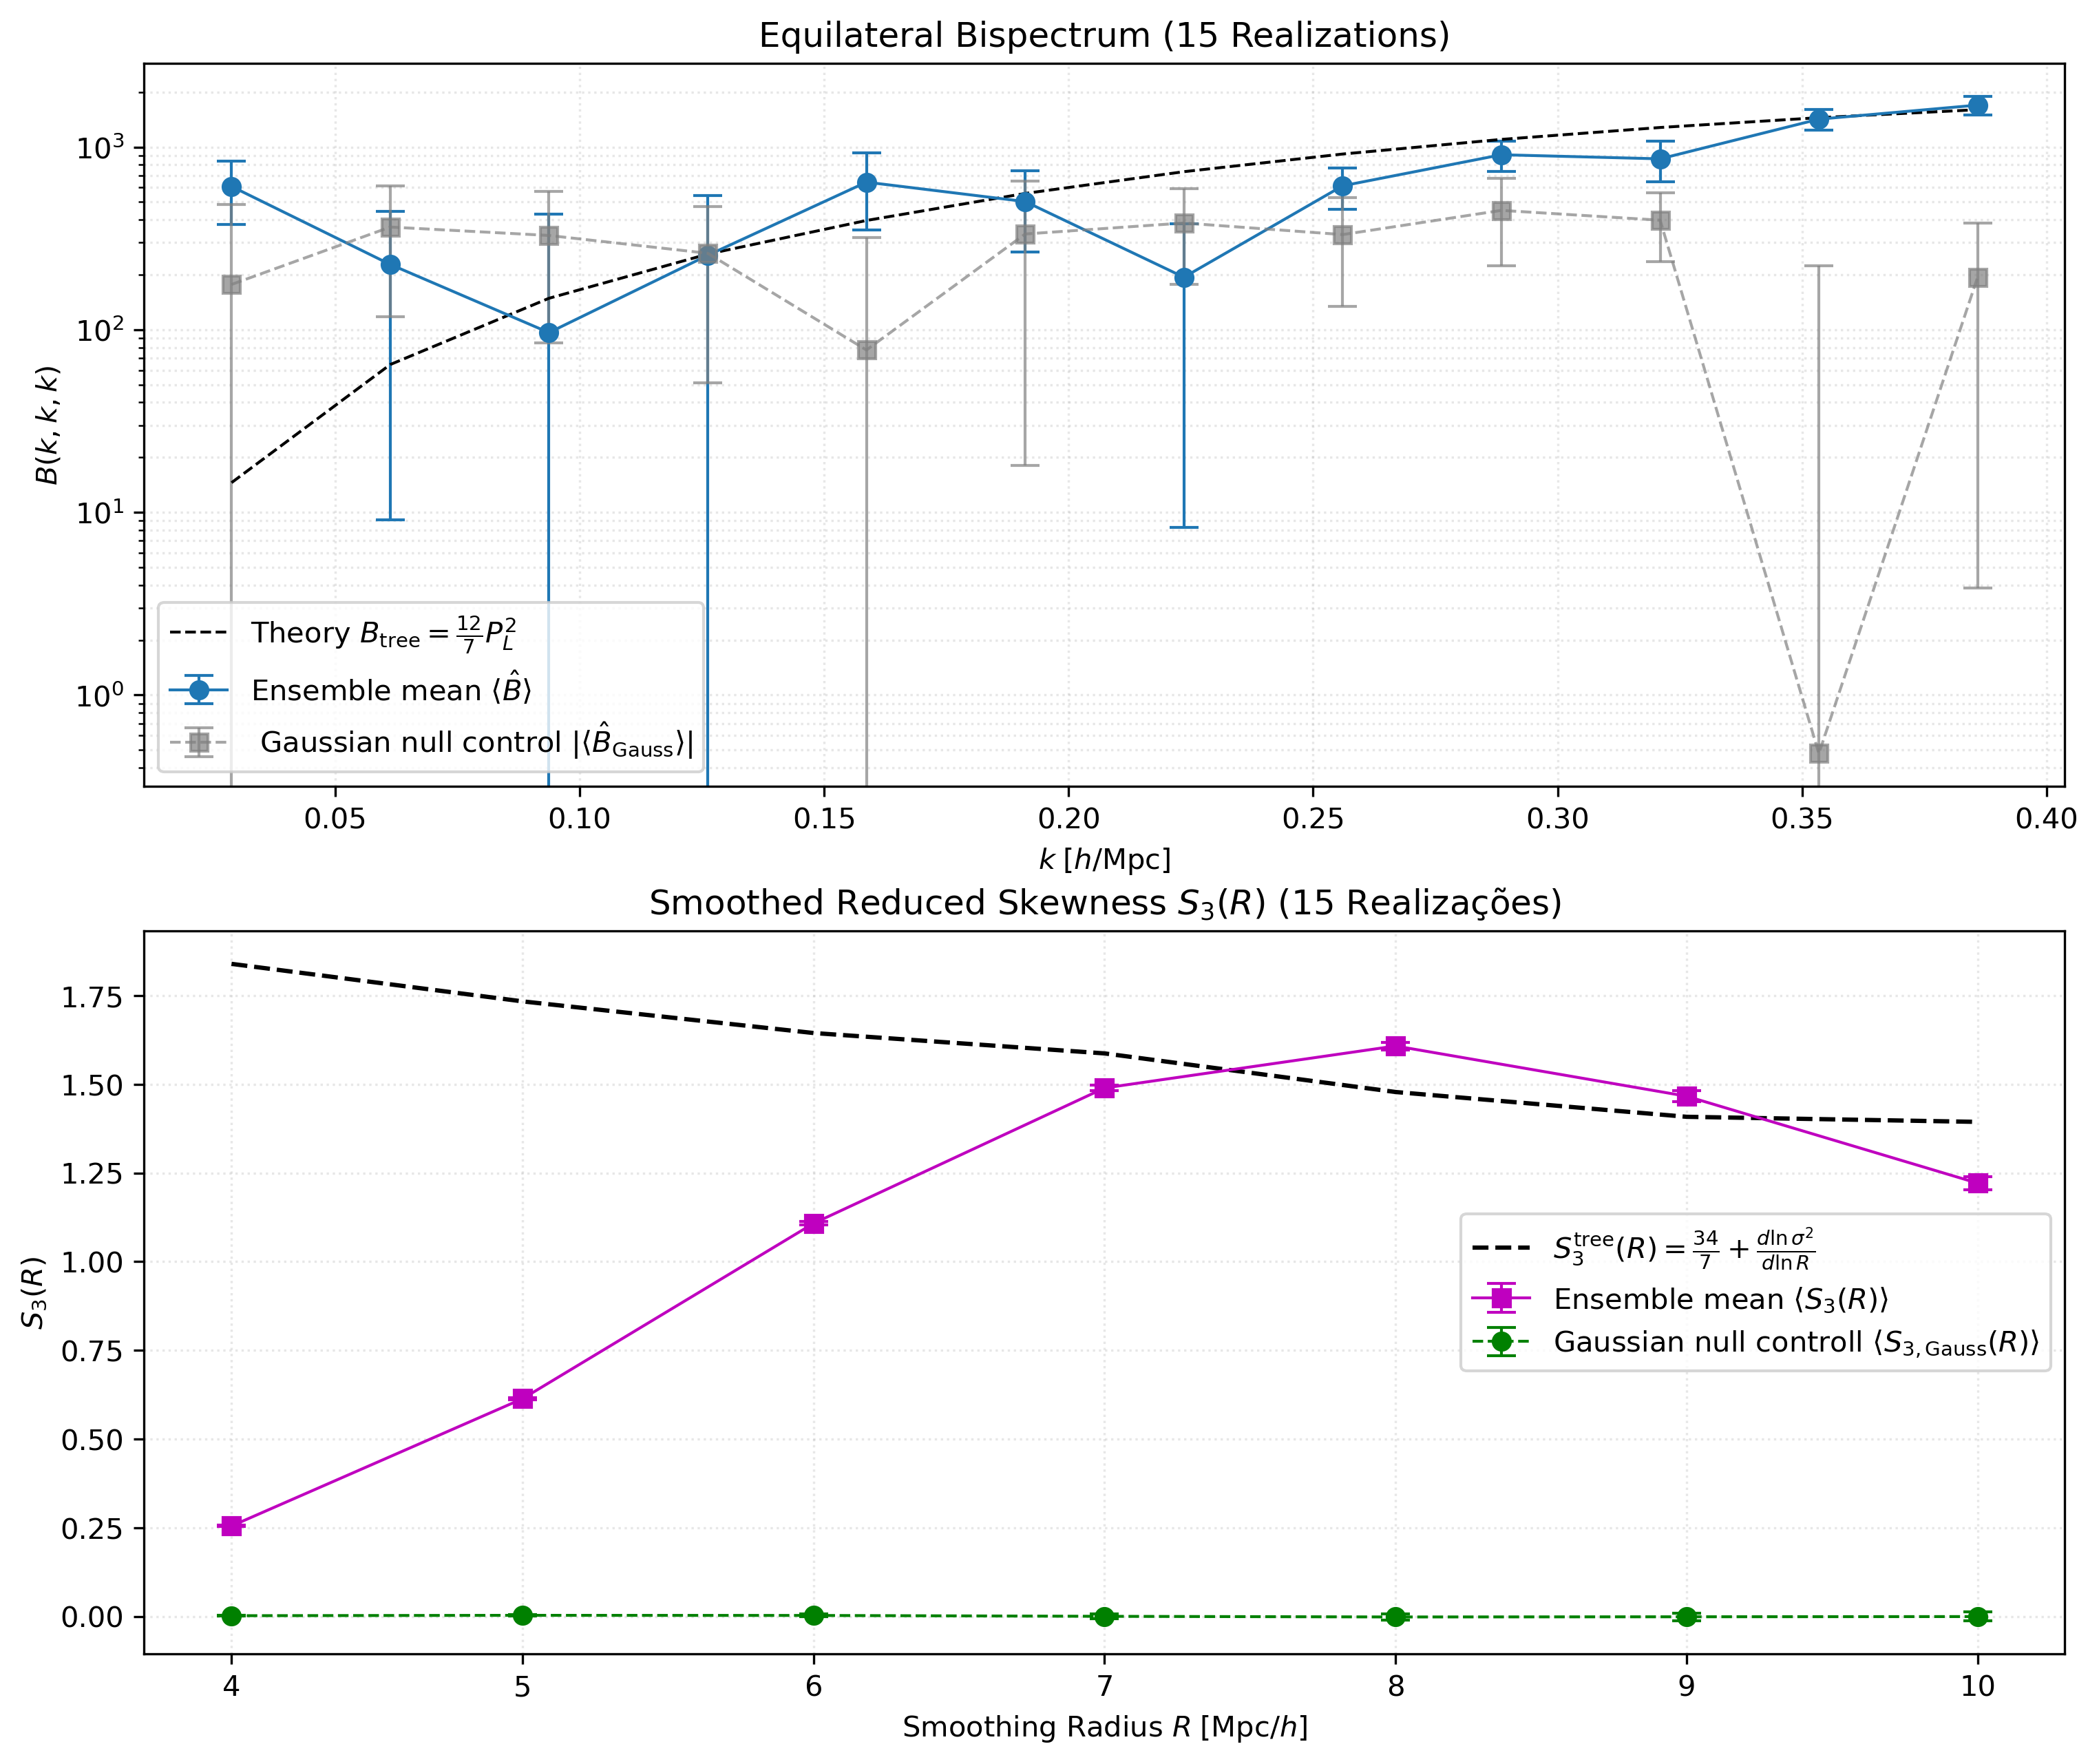
\includegraphics[width=0.7\linewidth]{New_Figures/Test_20261106_190746_Bispectrum_S3R_ensemble.png}
        \caption{Equilateral bispectrum $\langle \hat{B}(k,k,k) \rangle$ and smoothed reduced skewness $\langle S_3(R) \rangle$ averaged over 15 independent realizations ($\sigma_1^2 = 4.6116 \times 10^{-3}$)}
        \label{fig:spt_ensemble}
    \end{figure}

In the weakly non-linear regime ($\sigma_1^2 \approx 4.6116 \times 10^{-3}$), the equilateral bispectrum $B(k,k,k)$ across 12 wave-number bins and the Top-Hat smoothed reduced skewness $S_3(R)$ across $R \in [4, 10]\,h^{-1}\mathrm{Mpc}$ were evaluated.

As shown in Figure~\ref{fig:spt_ensemble}, averaging the equilateral bispectrum over an ensemble of $N_{\mathrm{real}} = 15$ independent realizations reduces single-box sampling scatter. The ensemble mean broadly follows the tree-level SPT expectation $B_{\mathrm{tree}}^{\mathrm{equil}}(k) = (12/7)P_L^2(k)$, with better agreement at higher wave numbers, although noticeable deviations remain across some intermediate modes.

\subsubsection{Box sensibility}

As a validation test, we investigate the sensitivity of the bispectrum and the reduced skewness to the simulation box size and spatial resolution. The results of these tests are summarized in the following figures:

\begin{figure}[H]
\centering
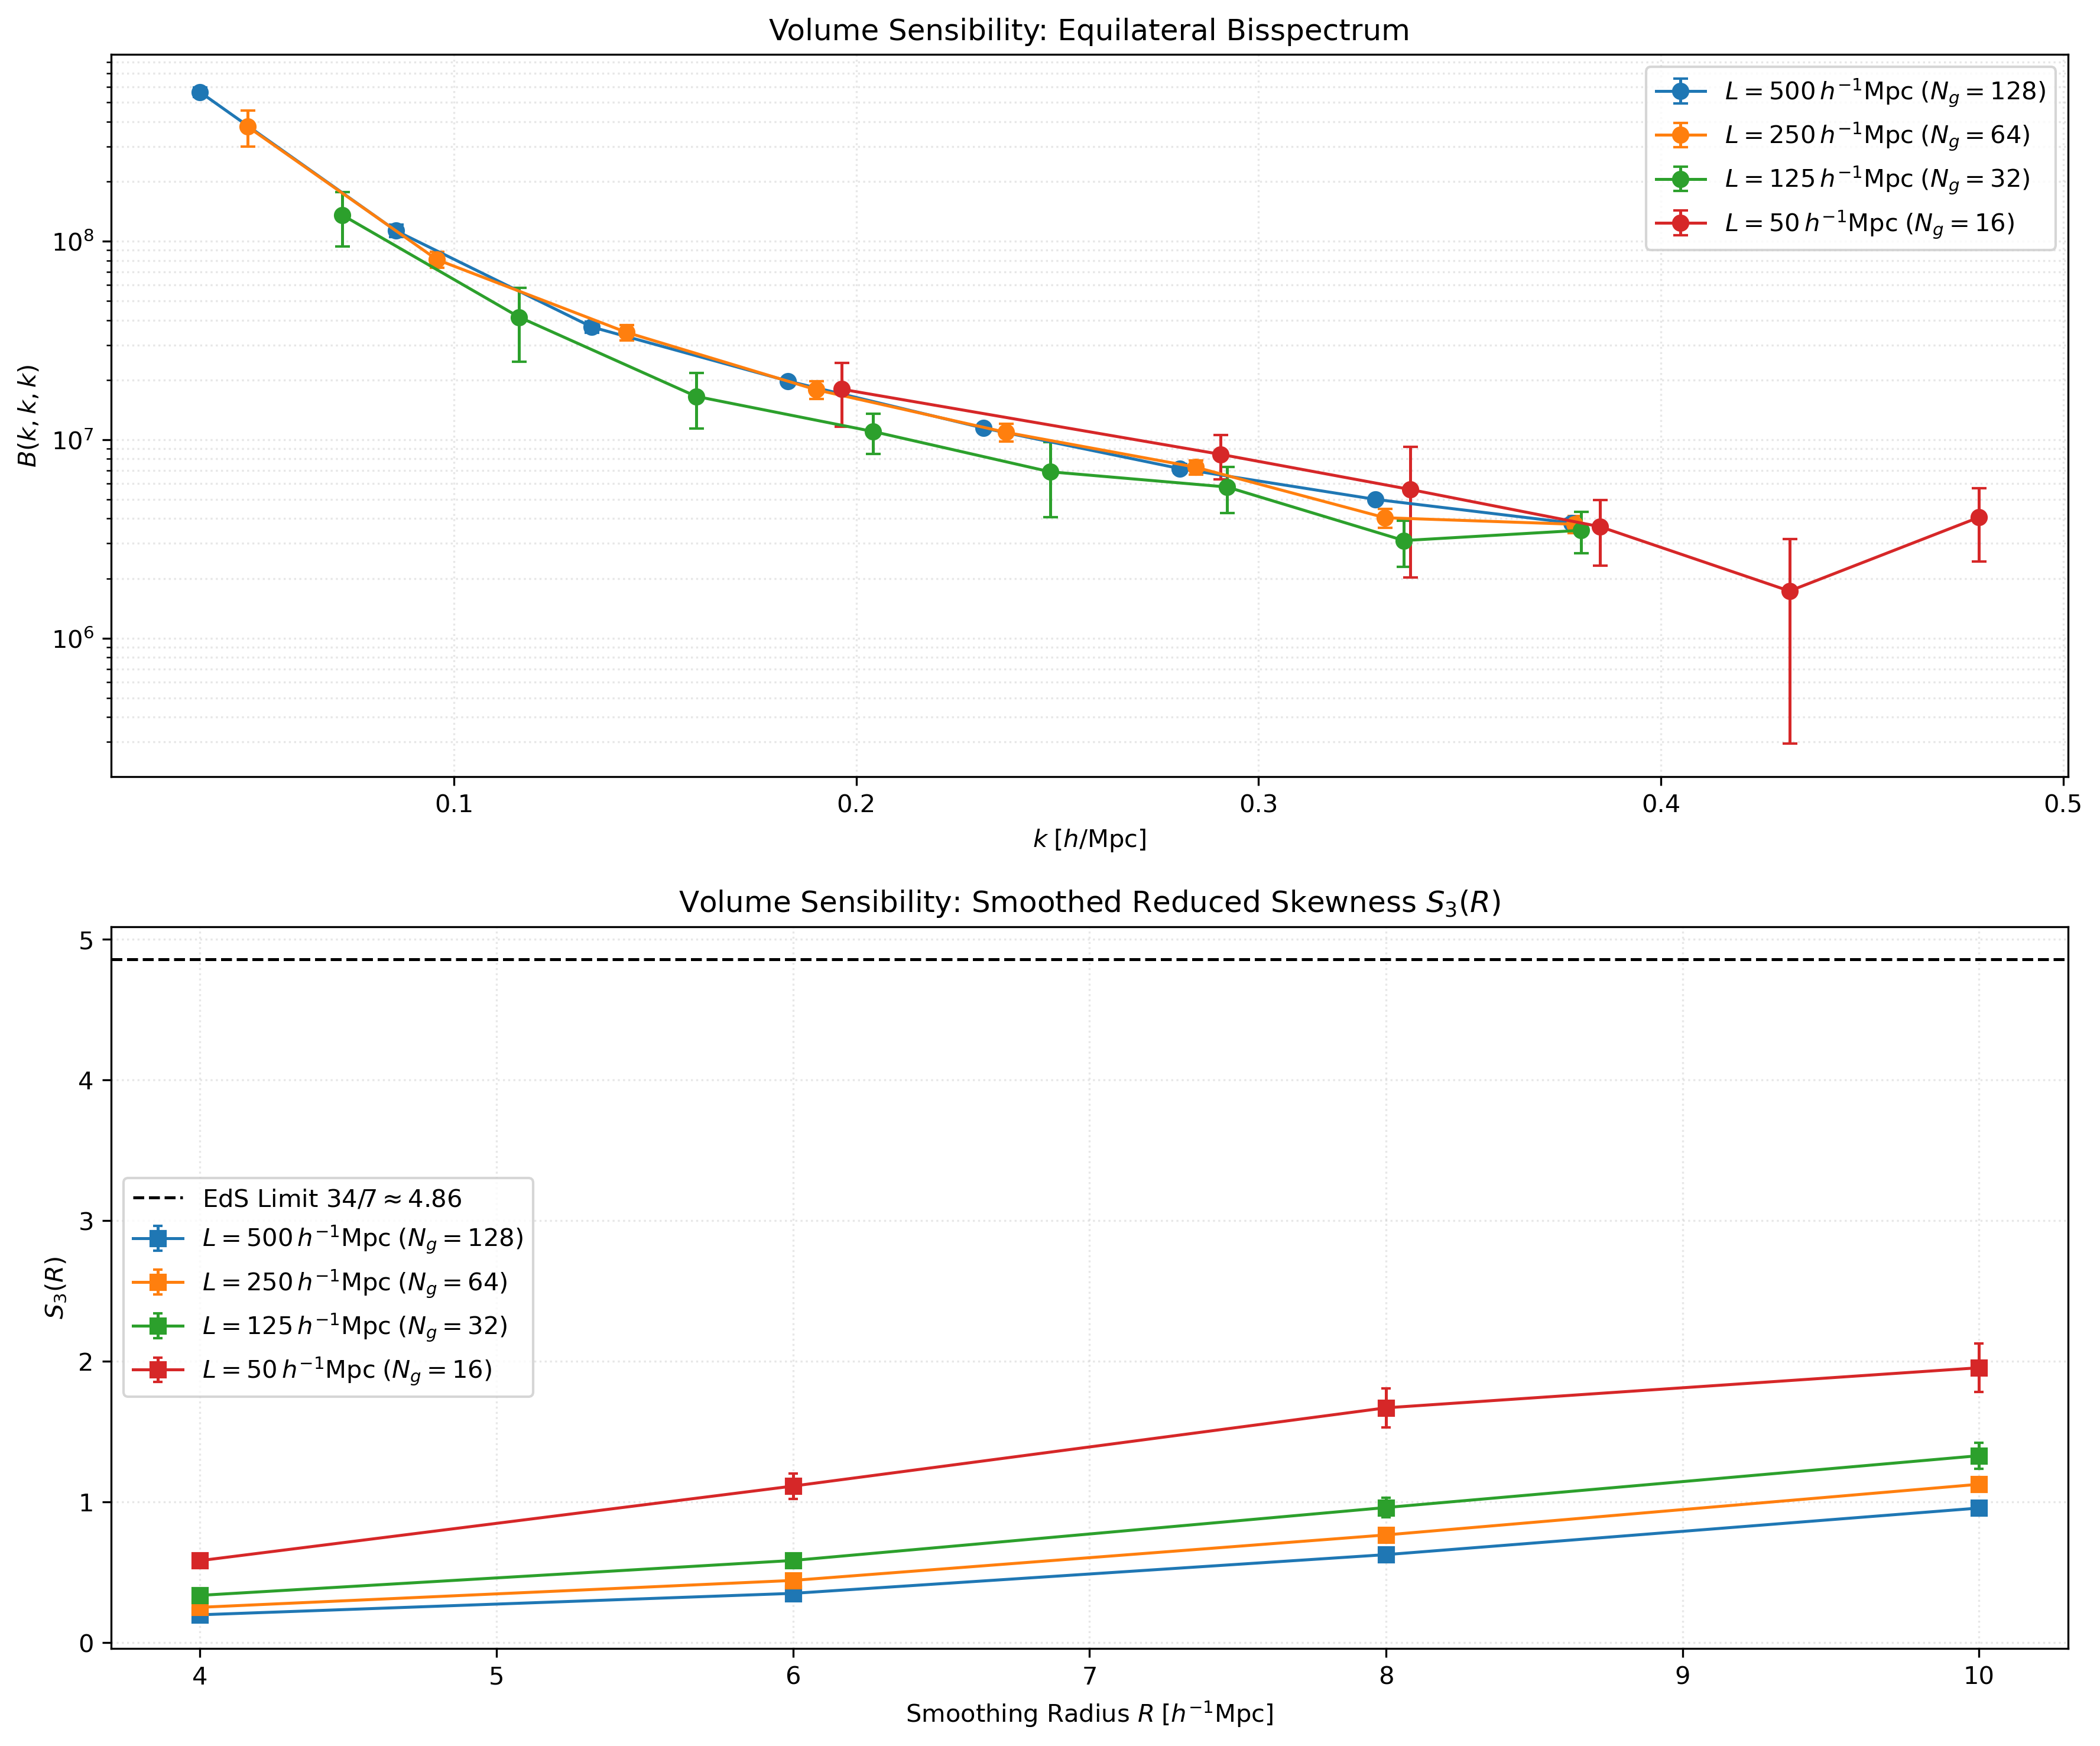
\includegraphics[width=0.7\linewidth]{New_Figures/Test_20261107_171604_Volume Sensibility_ Smoothed Reduced Skewnesse.png}
\caption{Volume sensitivity of the equilateral bispectrum $\langle \hat{B}(k,k,k) \rangle$}
\label{fig}
\end{figure}

For the volume sensitivity, the upper panel shows that the equilateral bispectrum exhibits an overall decreasing trend with increasing wavenumber. At low and intermediate wavenumbers, the scales are less affected by volume effects. At high wavenumbers, there are more discrepancies, indicating increased statistical fluctuations due to the limited number of available modes. In the lower panel, it is possible to see a dependence on the volume: smaller volumes produce larger values of $S_3(R)$, whereas the largest volume yields the lowest values. All the measurements are below the EdS limit.

\begin{figure}[H]
\centering
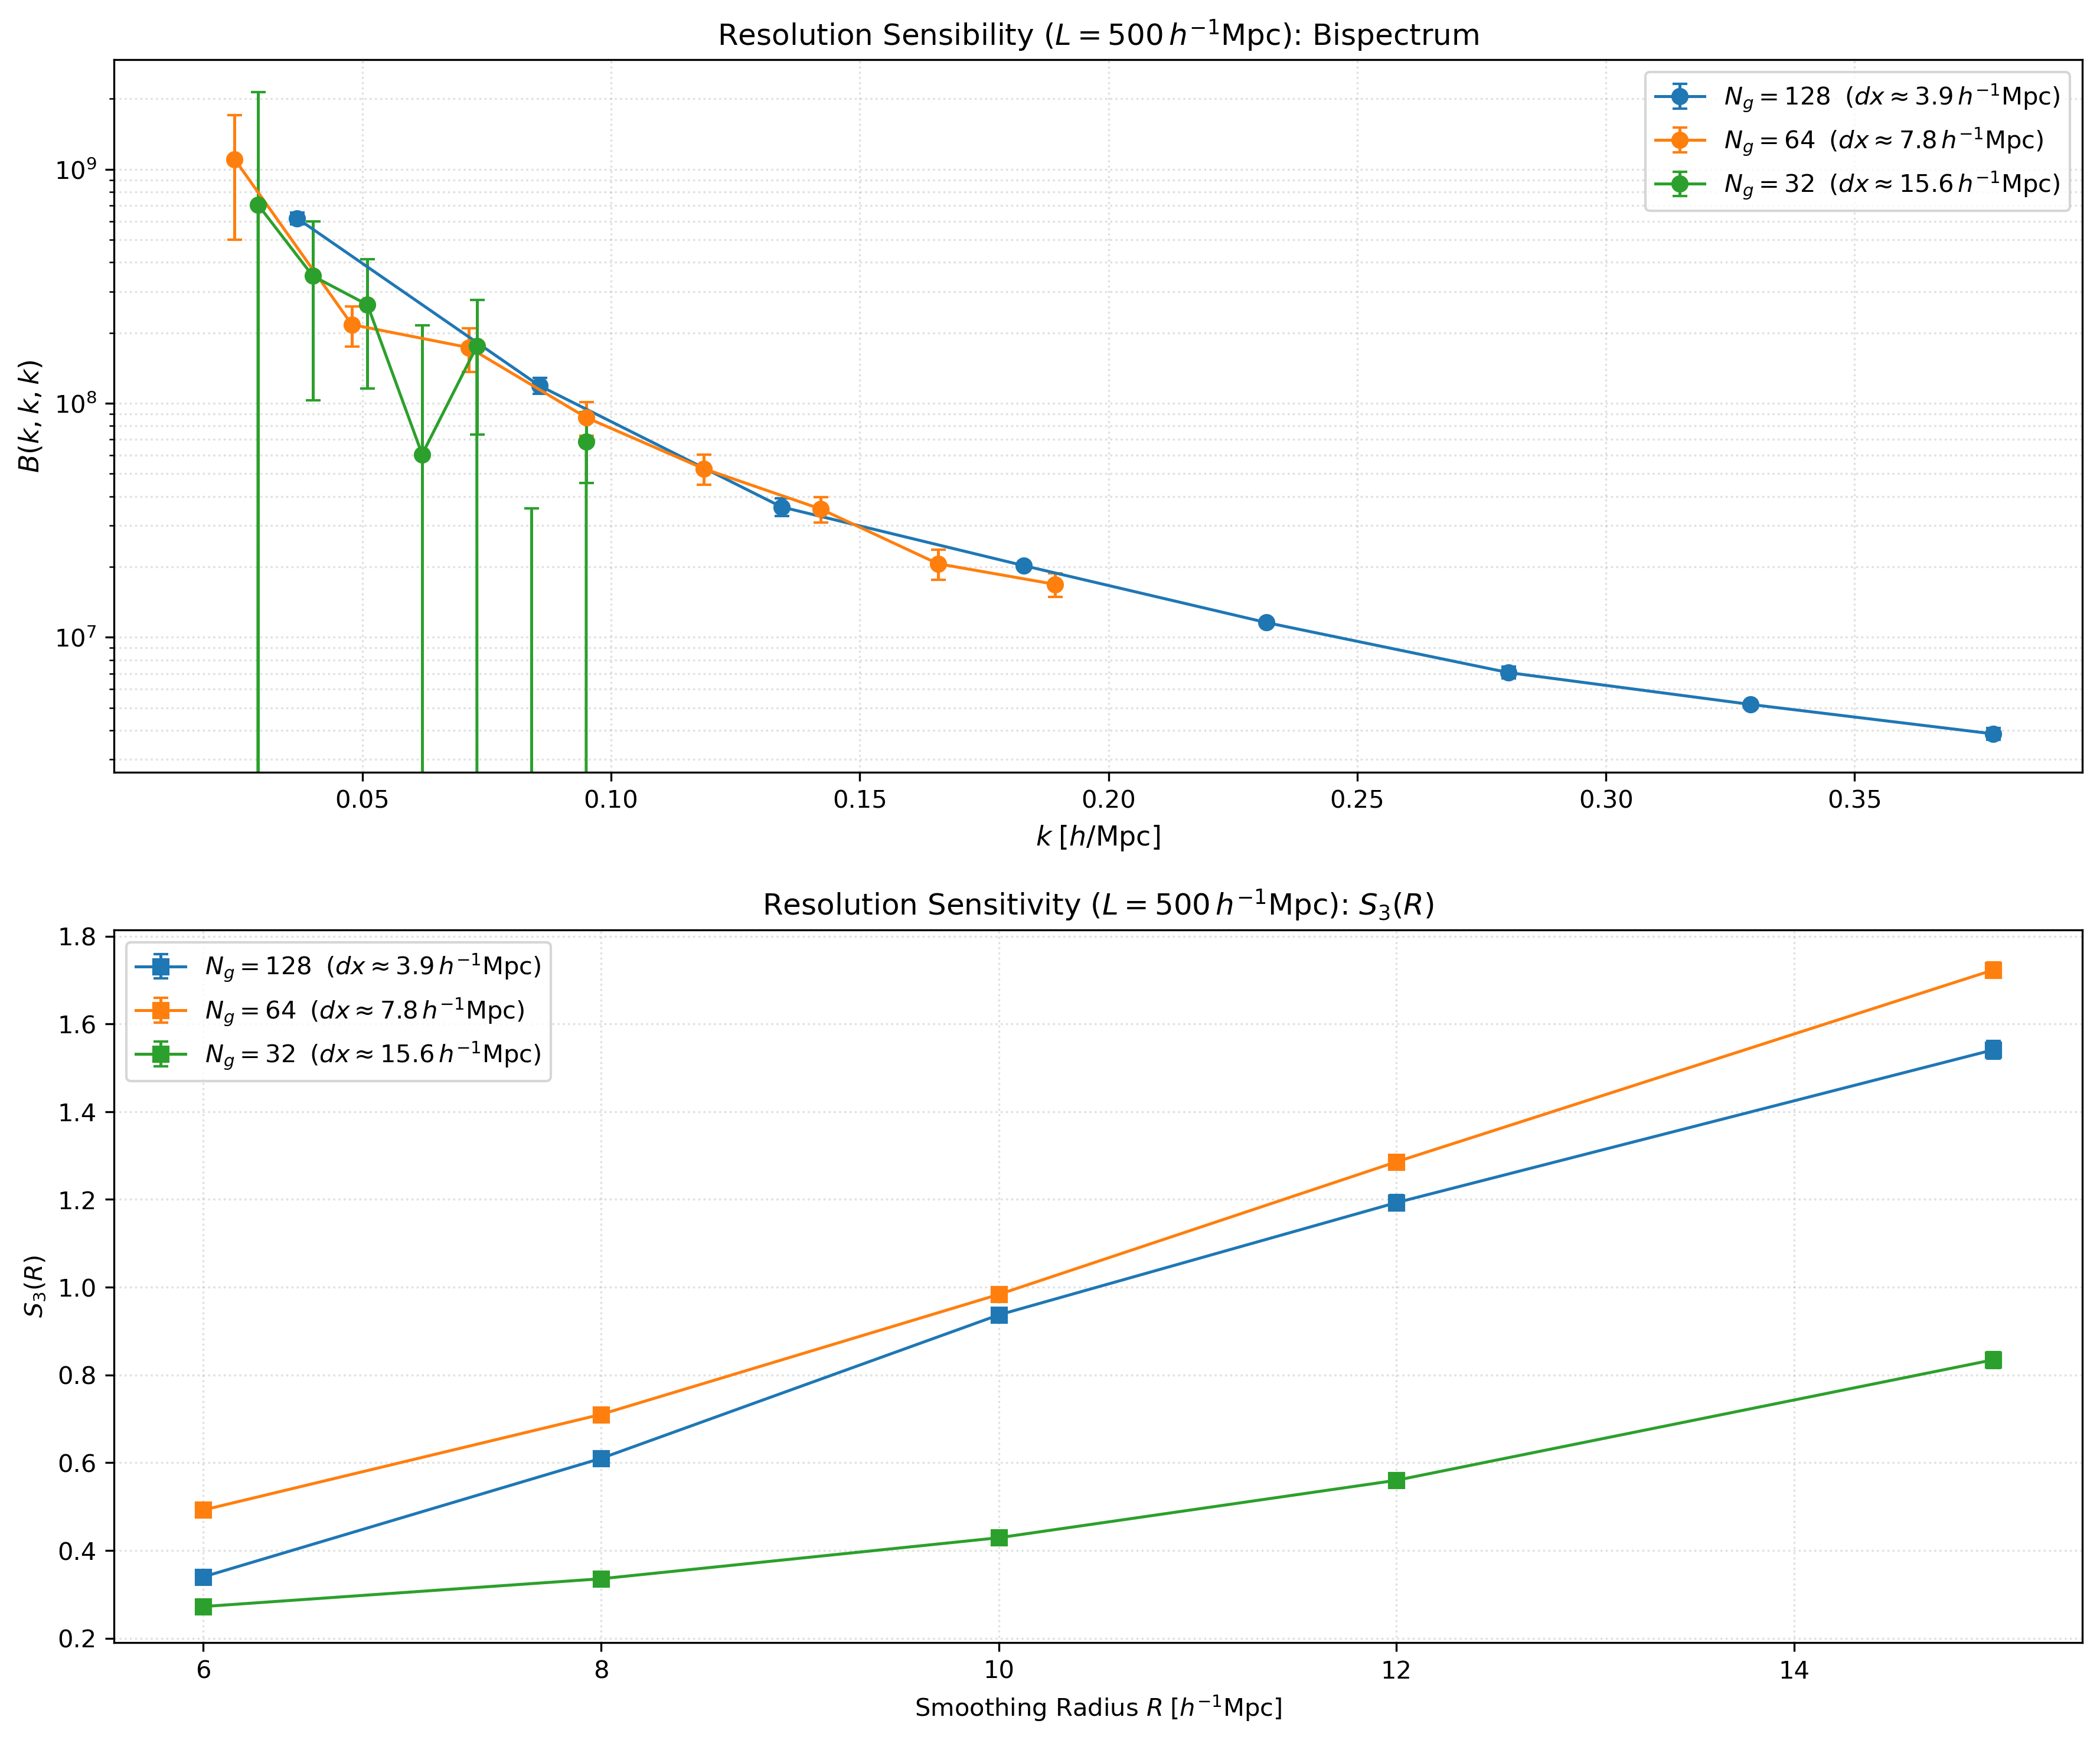
\includegraphics[width=0.7\linewidth]{New_Figures/Test_20261107_171604_Resolution_Sensitivity.png}
\caption{Resolution sensitivity of the equilateral bispectrum}
\label{fig}
\end{figure}

This figure shows the resolution sensitivity, where it is possible to see that the spatial resolution is a determining factor for higher-order statistical measurements. Although the two finer resolutions provide more consistent bispectrum estimates over their common range, noticeable differences remain in the reduced skewness.
